\addcontentsline{toc}{subsubsection}{\strut \hspace{24mm} 空间平均}

\vspace{\baselineskip} 
\vspace{\baselineskip} 
\noindent {\bf 空间平均}

\opthead{PR3}{\ws}{H. L. Tolman}


上述 GSE 缓解方法的主要缺点，是它可能影响模式经济性；这与式~(\ref{eq:ddif_4}) 有关，并在 \cite{tol:Waves01a,tol:OMOD02b} 中有讨论。因此，\ws\ 又开发了一种替代的附加 GSE 缓解方法。

该方法是 \ws\ 的默认方法，它用一个单独的分步替代附加扩散步骤 (\ref{eq:d_bal_1})；在该分步中，对给定谱分量的能量密度场进行直接平均。每个网格点周围用于平均的区域，在传播方向 ($\bs$) 和法向方向 ($\bn$) 上分别延伸为

\begin{equation}
\pm \gamma_{a,s} \: \Delta c_g \: \Delta t \: \bs \:\:\: ,
\pm \gamma_{a,n} \: c_g \Delta \theta \: \Delta t \: \bn \:\:\: , \label{eq:GSE_avg}
\end{equation}

\noindent
其中 $\gamma_{a,s}$ 和 $\gamma_{a,n}$ 为可调常数，默认值设为 1.5。该平均过程如图~\ref{fig:GSE_1} 所示。注意，如 \cite{tol:OMOD02b} 所讨论，在实际应用中这些值可能需要重新调整。该文附录 A 给出了平均格式的细节，包括守恒性方面的考虑。此外，与 \cite{art:BH87} 方法保持一致意味着 $\gamma_{a,s}$ 和 $\gamma_{a,n}$ 应随空间网格分辨率变化 \citep[见][Appendix]{tol:OMOD08a}。

注意，具有主导方向 $\bs$ 和 $\bn$ 的这种平均类似于 \cite{art:BH87} 的扩散方法，后者使用相同主方向。然而，该平均方法绝不会影响时间步长，因为它与实际传播完全分离。此外，如果使用显式格式，通常有 $c_g \Delta t / \Delta x < 1$，那么显然按 (\ref{eq:GSE_avg}) 定义的区域进行平均，一般只需要直接相邻空间网格点的信息，如图~\ref{fig:GSE_1} 所示。此外，该方法不需要高纬度滤波。

\begin{figure} \begin{center}
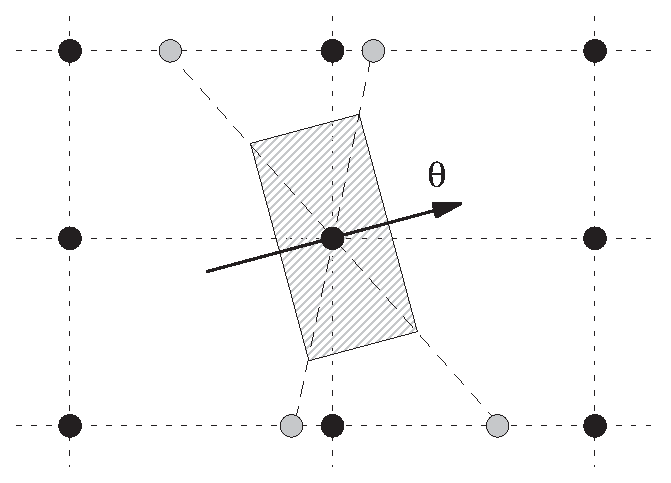
\epsfig{file=./num/GSE_1.eps,angle=0,width=2.2in}
\caption{空间平均 GSE 缓解技术示意图。实心圆和虚线表示空间网格。阴影区域表示需要考虑的平均区域。角点值由中心网格点和灰色点得到；后者通过相邻网格点插值得到 \citep[引自][]{tol:OMOD02b}。}
\label{fig:GSE_1} \botline
\end{center}
\end{figure}

如 \cite{tol:OMOD02b,tol:OMB02b} 所示，该方法给出的结果几乎与前一种方法相同，但计算成本略低。对于高分辨率应用，平均方法可能显著更经济。



最后，通过保证离散谱方向不与空间网格线重合，也可在一定程度上缓解 GSE。这可通过把第一个离散方向 $\theta_1$ 定义为

% eq:theta1          First direction

\begin{equation}
\theta_1 = \alpha_\theta \: \Delta \theta \:\:\: , \label{eq:theta1}
\end{equation}

\noindent
其中 $-0.5 \leq \alpha_\theta \leq 0.5$ 可由用户定义。注意，设置 $\alpha \neq 0$ 有利于一阶格式，但对三阶格式影响可忽略。
 
